\section{Software Architecture of the model}
% Start here

\subsection{Introduction}

The first step when developing a Classical B  model is to define the architecture of the software to model.

The language allows to give a structure to the model close to the one of the software implemented.
Thus functions are shared between components : those in charge of scheduling the functions, those in charge of managing the inputs, those in charge of managing the output, those in charge of describing the functions in details...  This allows a modular development of the software.

In Classical B, to describe a function (or a set of functions) we need at least two components :  an abstract machine which gives an abstract specification of the functions, and an implementation to detail the functions as an implementable code (by convention the implementation has the same name as the abstract machine with the suffix "\_i"). As much refinement components as necessary can be added between an abstract machine and an implementation to refine step by step the abstract specification until the implementation and to facilitate traceability. Refinement components are usually used only in the case of complex functions. This is the first mean to structure a Classical B model with abstraction level (this can be compared with the distinction between spec and body components of language such as C, Ada or Java).

The second means to structure the Classical B  models is to link the group of components together. Then in a given machine or implementation :
\begin{description}
\item[the SEES clause] allows to link the components which can be viewed in the component : Variables can be read but not modified (it works as "with" clause in C, Ada or Java software)
\item[the IMPORT clause] allows to link the components whom variables can be modified with call of functions (it works as "use" clause in C, Ada or Java software).
\end{description}


\subsection{ETCS  case study}


Figure \ref{fig:graphe} gives the architecture of the ETCS example developed during benchmark activities. Arrows show IMPORT relations.

 \begin{figure}
  \centering
  \fbox{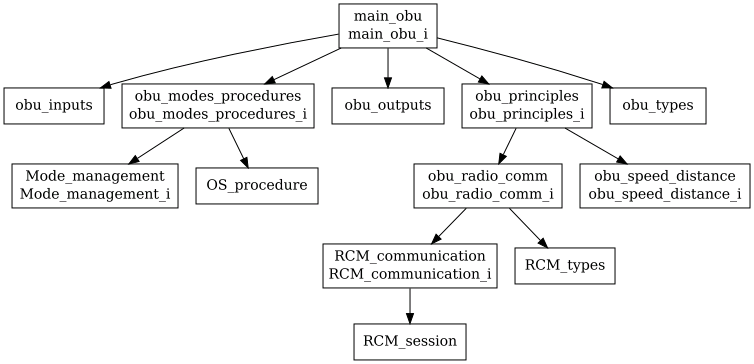
\includegraphics[scale=0.75]{graphe.png}}
  \caption{Classical B  model architecture}
  \label{fig:graphe}
\end{figure}


\begin{description}
\item[main\_obu] is the main sequencer of the software
\item[obu\_types] contains the definition of types and constants used by all the software components. This machine is seen by all the other components.
\item[obu\_inputs] stores the input values in different variables. This machine is seen by most of the other components.
\item[obu\_outputs] manages the outputs.
\item[obu\_modes\_procedures] and branches below are in charge of the management of modes and procedures (subset 26 chapter 4 and 5).
\item[obu\_principles] and branches below are in charge of the functions (chapter 3 of subset 26).
\end{description}

\subsubsection{Main sequencer}

This is the main sequencer with two operation called by the hardware. We assume an applicative cycle is defined and at each cycle the main operation "cycle" is called. The operation "power\_up" is called when the system is started.

\fbox{
\begin{minipage}{14cm}

\bf MACHINE

\hspace*{0.20in}\it main\_obu

\hspace*{0.20in}

\hspace*{0.20in}\bf OPERATIONS

\hspace*{0.20in}

\hspace*{0.20in}\bf power\_up \rm =

\hspace*{0.20in}\bf BEGIN

\hspace*{0.40in}\bf skip

\hspace*{0.20in}\bf END \rm ;

\hspace*{0.20in}

\hspace*{0.20in}\bf cycle \rm =

\hspace*{0.20in}\bf BEGIN

\hspace*{0.40in}\bf skip

\hspace*{0.20in}\bf END

\vspace*{12mm}
\bf END
\end{minipage}
}

\vspace*{8mm}

The implementation gives the sequence of the main operations called at each cycle and during the initialisation. first the inputs at read (we assume here the inputs are read  and stored at the beginning of each cycle and not on the fly). The called operation are defined in the imported components.


\fbox{
\begin{minipage}{14cm}


\bf IMPLEMENTATION

\hspace*{0.15in}\it main\_obu\_i

\bf REFINES

\hspace*{0.20in}\it main\_obu

\vspace*{4mm}
\bf IMPORTS

\hspace*{0.20in}\it obu\_inputs\rm ,

\hspace*{0.20in}\it obu\_modes\_procedures\rm ,

\hspace*{0.20in}\it obu\_principles\rm ,

\hspace*{0.20in}\it obu\_outputs\rm , 

\hspace*{0.20in}\it obu\_types

\vspace*{4mm}
\bf OPERATIONS

\hspace*{0.15in}\bf power\_up \rm =

\hspace*{0.15in}\bf BEGIN

\hspace*{0.35in}\bf initial\_read\_inputs \rm ;

\hspace*{0.35in}\bf intialize\_mode \rm ; \hspace*{0.35in}

\hspace*{0.35in}\bf initialize\_data \rm ; \hspace*{0.35in}

\hspace*{0.35in}\bf initial\_send\_outputs

\hspace*{0.15in}\bf END

\hspace*{0.15in}\rm ;

\vspace*{4mm}
\hspace*{0.15in}\bf cycle \rm =

\hspace*{0.15in}\bf VAR \it vv \bf IN

\hspace*{0.35in}\bf read\_inputs \rm ;

\hspace*{0.35in}\it vv  $\leftarrow$  \bf get\_V\_train \rm ;

\hspace*{0.35in}\bf modes\_procedures\_management\rm (\it vv\rm ) \rm ; \hspace*{0.75in}

\hspace*{0.35in}\bf principles\_management \rm ; \hspace*{0.20in}

\hspace*{0.35in}\bf send\_outputs

\hspace*{0.15in}\bf END

\vspace*{8mm}
\bf END

\end{minipage}
}


\vspace*{8mm}

\subsubsection{Types}

The component obu\_types  defines the types and constants used by the whole system as modes, level,..

\fbox{
\begin{minipage}{14cm}


\bf MACHINE

\hspace*{0.20in}\it obu\_types

\hspace*{0.20in}

\bf SETS

\it t\_mode \rm = \rm \{\it FS\rm , \it LS\rm , \it OS\rm , \it SR\rm , \it SH\rm , \it UN\rm , \it PS\rm , \it SL\rm , \it SB\rm , \it TR\rm , \it PT\rm , \it SF\rm , \it ISo\rm , \it NP\rm , \it NL\rm , \it SN\rm , \it RV\rm \}

\rm ;

\it t\_mamode \rm = \rm \{\it ma\_OS\rm , \it ma\_SH\rm , \it ma\_LS\rm , \it ma\_unknown\rm \}

\rm ;

\it t\_level \rm = \rm \{\it level\_0\rm , \it level\_1\rm , \it level\_2\rm , \it level\_3\rm , \it level\_NTC\rm \}

\rm ;

\it t\_procedure \rm = \rm \{\it NoProcedure\rm , \it StartOfMission\rm , \it EndOfMission\rm , \it SHInitiatedByDriver\rm ,

 \it SHOrderFromTrackside\rm , \it Override\rm , \it OnSight\rm , \it LevelTransitions\rm , \it TrainTrip\rm , 
 
 \it ChangeTrainOrientation\rm , \it TrainReversing\rm , \it Joining\rm , \it Splitting\rm , \it RBCHandover\rm , 
 
\it LevelCrossing\rm , \it ChangingTrainData\rm , \it TrackConditions\rm , \it LimitedSupervision\rm \}

\vspace*{4mm}
\bf CONSTANTS

\hspace*{0.20in}\it VITESSE

\hspace*{0.20in}

\bf PROPERTIES

\hspace*{0.20in}\it VITESSE  $\subseteq$  \bf NAT  $\land$ 

\hspace*{0.20in}\it VITESSE \rm = \rm 0 $\upto$ \rm 6\rm 0\rm 0

\vspace*{4mm}
\bf END

\end{minipage}
}

\newpage


